\documentclass{beamer}
\usepackage[T1]{fontenc}
\usepackage[spanish]{babel}
\usetheme{Boadilla}
\title{Proyecto de programacion}
\author{Adrián Alejandro Souto Morales}
\begin{document}
    \begin{frame}
        \begin{figure}
            \centering
            
\includegraphics[width = 3cm]{img/searchbar.png}
        \end{figure}
        \maketitle
        C-122
    \end{frame}
    \begin{frame}
        \frametitle{MoogleServer/Program.cs}
        En \textit{MoogleServer/Program.cs} se llama a la función \textbf{GetData()} que carga todos los datos necesarios que se ejecuta mientras se monta el servidor:
    \\
        \begin{figure}[h]
            \centering
            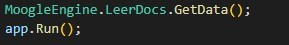
\includegraphics[width = 9cm]{img/MoogleServer.jpg}
            \caption[]{Fragmento de MoogleServer.cs}
        \end{figure}
        
    \end{frame}

    \begin{frame}
        \frametitle{LeerDocs}
        La clase estática \textbf{“LeerDocs”} contiene la función \textbf{“GetData()”} para crear un \textbf{“Vector”} por cada 
        documento con las respectivas palabras que lo componen.
        \begin{figure}[h]
            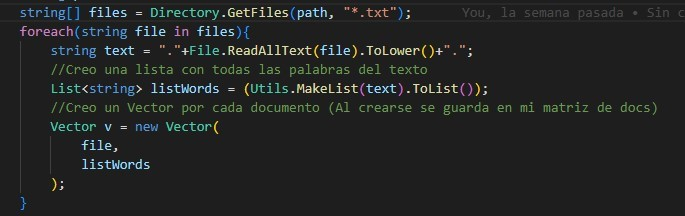
\includegraphics[width = 9cm]{img/LeerDocs.jpg}
            \caption[]{Función de GetData()}
        \end{figure}  
    \end{frame}
    \begin{frame}
        \frametitle{Vector}
        \textbf{\\\large{Propiedades:}}
        \begin{itemize}
            \item \textbf{TFIDF} (Dictionary$<$string, double$>$)
            \item \textbf{Path} (string)
            \item \textbf{Words} (List$<$string$>$)
        \end{itemize}
        \textbf{\\\large{Métodos:}}
        \begin{itemize}
            \item  \textbf{CountWords()}
            \item \textbf{GetName()}
            \item  \textbf{ProdEscalar(Vector v)}
        \end{itemize}
    \end{frame}
    \begin{frame}
        \frametitle{Matriz}
        \textbf{\\\large{Propiedades:}}
        \begin{itemize}
            \item  \textbf{MatrizVectores}(List\textit{$<$Vector$>$})
            \item \textbf{IDF}(Dictionary\textit{$<$string, int$>$})
        \end{itemize}
        \textbf{\\\large{Métodos:}}
        \begin{itemize}
            \item  \textbf{Add}(Vector v)
            \item \textbf{CalculateIDF}(string w)
            \item \textbf{CalculateTF}(Vector v, string w)
        \end{itemize}
    \end{frame}
    \begin{frame}
        \frametitle{Search}
        La función \textbf{Search()} ubicada en la clase Moogle.cs retorna un array de \textbf{SearchItem}:
    
        \begin{enumerate}
            \item \textbf{Calcula el score} por cada vector y solo lo muestra si es mayor a $10^-6$ (Producto 
            escalar entre el query y el vector)
            \item Guarda la posición de la palabra con más TF-IDF del query que esté en el documento
            \item \textbf{Guarda el snippet} dado por un fragmento del texto que contenga dicha palabra
            (Desde punto (“.”) anterior a 50 caracteres antes de la palabra hasta el 
            siguiente punto después de 100 caracteres)
            Para ello se usan las funciones NextDot() y PrevDot() de mi clase Utils.
            \item Guarda en una Lista de SearchItem los datos del vector (nombre, snippet, score)
            \item Cuando termina de recorrer los vectores ordena la Lista de SearchItem según su score, 
            la convierte en Array y la devuelve    
        \end{enumerate}
    \end{frame}
    \begin{frame}
        \frametitle{Utils}
        \textbf{\\\large{Métodos:}}
        \begin{itemize}
            \item  \textbf{MakeList}(string text)
            \item \textbf{PrevDot}(int pos, string text)
            \item \textbf{NextDot}(int pos, string text)
        \end{itemize}
    \end{frame}
    

\end{document}